\newtoggle{withbonus} \togglefalse{withbonus} % set true to show bonus points in grade table

% setting underlying course name (Grundlagenfach Mathematik, §-Unterricht, \ldots)
\newcommand{\mycourse}{Grundlagenfach Geografie}
% name of the class
\newcommand{\myclass}{G22s}
% set date
\newcommand{\mydate}{11. März 2025}

\title{\textbf{Prüfung: Stadtgeografie}}
\author{Niklaus Lusser, Cyril Wendl\\
	\mycourse, \myclass}
\date{\mydate}
\maketitle
\thispagestyle{headandfoot}

\begin{center}
	\fbox{\parbox{140mm}{\centering
			\begin{itemize}
				\item Dauer der Prüfung: $45$ Minuten
				      %\item \textbf{Zeige in jeder Aufgabe unbedingt Deine Schritte!}
				\item Erlaubte Hilfsmittel:
				      \begin{itemize}
					      \item Schreibzeug
					      \item Farbstifte
					      \item Leuchtstifte
				      \end{itemize}
			\end{itemize}}}
\end{center}
\vspace{10mm}

\begin{center}
	Vorname: \rule{45mm}{0.8pt}\qquad Nachname: \rule{45mm}{0.8pt}
\end{center}
\vspace{20mm}

\begin{center}
	\iftoggle{withbonus} {
		\combinedgradetable[h][questions]
	} {
		\gradetable[h][questions]
	}
\end{center}
\vspace{15mm}
\begin{center}
	Note:
	\vspace{10mm}

	\rule{8mm}{1.2pt}
\end{center}
%\thispagestyle{empty}
\clearpage

\begin{questions}
	\section*{\textcolor{Green}{Entwicklungsphasen der europäischen Stadt}}
	\question Auf folgendem Luftbild der Stadt Solothurn erkennen Sie drei eingefärbte Gebiete (orange, rot, blau). 
			\begin{figure}[H]
			\centering
			\includegraphics[width=\linewidth, page=1,trim={4.5cm 4.7cm 1cm 1cm},clip]{"Geografie/Exam/Karte Solothurn.pdf"}
			\end{figure}
	Erläutern Sie für jedes dieser Gebiete:
	\begin{parts}
		\part[3] Name der städtebaulichen Phase:
		\fillwithlines{4cm}
		\begin{solution}
		\begin{itemize}
		\item Oranges Gebiet: Industrialisierung
		\item Rotes Gebiet: Mittelalter
		\item Blaues Gebiet: Neuzeit / Gegenwart
		\end{itemize}
		\end{solution}
		\part[3] Ungefähre zeitliche Einordnung der Städtebau-Phase:
		\fillwithlines{4cm}
		\begin{solution}
		\begin{itemize}
		\item Oranges Gebiet: 19. - 20. Jahrhundert
		\item Rotes Gebiet: 8. - 15. Jahrhundert
		\item Blaues Gebiet: 20. / 21. Jahrhundert
		\end{itemize}
		\end{solution}
		\clearpage
		\part[3] Ein räumliches Erkennungsmerkmal der städtebaulichen Periode:
		\fillwithlines{4cm}
		\begin{solution}
		\begin{itemize}
		\item Oranges Gebiet: Blockrandbebauung, Bahnhof in der Nähe
		\item Rotes Gebiet: Dichte, verwinkelte Überbauung, ``chaotischer'' / verschachtelter Grundriss
		\item Blaues Gebiet: Einfamilienhäuser, Ausrichtung entlang Strassennetz, Netz aus Haupt- und Nebenstrassen
		\end{itemize}
		\end{solution}
	\end{parts}
	
	\droptotalpoints
	
	\bonusquestion[1] Oberhalb vom rot eingefärbten Gebiet sehen Sie einen Park. Wie könnte dieser entstanden sein?
	\fillwithlines{4cm}
	\begin{solution}
	Es handelt sich hierbei um einen Graben, auf dessen Grund sich früher die Zitadelle von Solothurn befand (s. eckige Formen im Park). Als diese nicht mehr benötigt wurde, wurde das ehemalige Festungs-Gebiet begrünt.
	\end{solution}
	\droptotalpoints
	\vfill
	\clearpage
	\question Folgende Fotos illustrieren charakteristisch die städtebaulichen Entwicklungen der europäischen Städte von der Nachkriegszeit (ca. 1950) bis ca. im Jahr 2000.
	
	\begin{figure}[H]
	\centering
	
\includegraphics[width=\linewidth]{Private/Images/peri}
	\end{figure}
	
	\begin{parts}
	\part[5] Welche Phase der Städteentwicklung könnte mit den obigen Bildern dargestellt sein? Nennen Sie drei Gründe, welche zu dieser Entwicklung geführt haben sowie zwei Folgen.
	\fillwithlines{4cm}
		
		\begin{solution}
		Notwendige Schlüsselbegriffe, um alle Punkte zu erhalten, sind fett markiert (Synonyme möglich): 
		
		Nach dem zweiten Weltkrieg führte ein \textbf{breiter wirtschaftlicher Aufschwung} sowie technologische Entwicklungen dazu, dass eine breite Bevölkerungsschicht Zugang zu \textbf{Automobilen} und damit verbundener Mobilität erhielten. Die \textbf{Lebensqualität} in den Städten war infolge der Industrialisierung und dem Aufkommen von Fabriken teilweise schlecht, so dass ein Leben auf dem Land attraktiver schien. Mit dem Automobil konnten lange Wege schnell zurückgelegt werden, so dass viele Menschen ein schönes Einfamilienhaus auf dem Land einer kleinen, engen Stadtwohnung bevorzugten. Hauptfolgen davon sind die \textbf{Zersiedelung} (grossflächige Überbauung) vieler Landschaften der Schweiz sowie die demografische \textbf{Verlagerung von städtischen und stadtnahen (suburbanen) Gebieten in entlegenere, ländlichere (periurbanere) Gebiete}.
			\end{solution}
			\part[4] Erklären Sie den Begriff ``\textbf{Reurbanisierung}'', indem Sie 2 Ursachen nennen, welche zur Reurbanisierung geführt haben, sowie 2 Massnahmen, um die Reurbanisierung voranzutreiben.
			\fillwithlines{4cm} 
			\begin{solution}
			\textbf{Mehrere Gründe möglich}:
			\begin{itemize}
			\item Sinkende Steuereinnahmen der Städte
			\item Tägliche zeitliche Einbussen durch Pendeln
			\item Mehrausgaben für Autobesitz
			\item Leben auf dem Land für gewisse Bevölkerungsschichten (Nachwuchs der Babyboomer) weniger attraktiv
			\end{itemize}
			
			\textbf{Massnahmen}:
			\begin{itemize}
			\item Finanzielle Anreize (günstiger Wohnraum): Grosswohnsiedlungen, Verdichtung gegen innen
			\item Förderung von ÖV innerhalb und zwischen den Städten
			\end{itemize}
			\end{solution}
	\end{parts}	
	
	\droptotalpoints
	\clearpage
	\question[6] Beschreiben Sie anhand des folgenden Bildes drei Arten von Segregation, welche sich in Städten vorfinden können, und erläutern sie, wie die jeweilige Segregationsart zustande kommt.
	
	\begin{figure}[H]
	\centering
	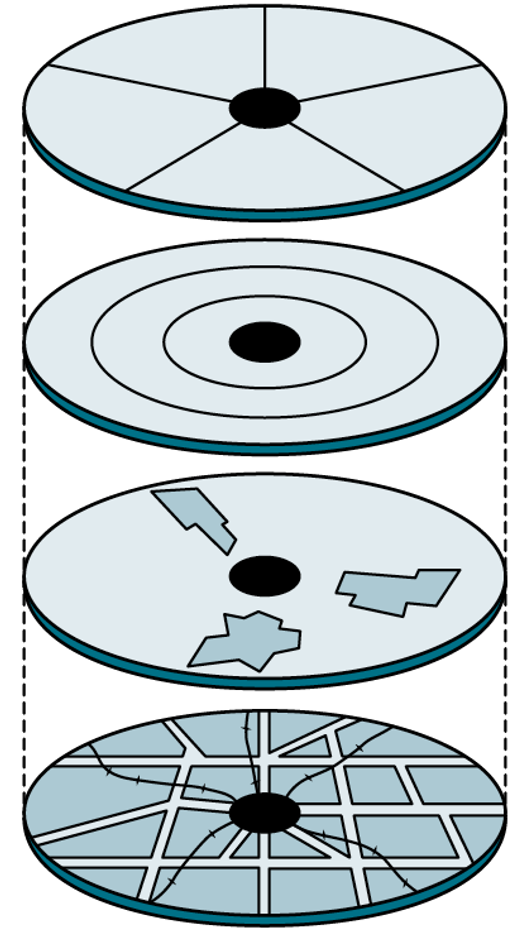
\includegraphics[width=0.2\linewidth]{Private/Images/segregationLeer}
	\caption{Segregationsarten (zuunterst: der physische Raum)}
	\end{figure}
	\fillwithlines{12cm}
	
	
	\begin{solution}
	\begin{itemize}
	\item \textbf{Soziale Segregation / Armutssegregation}: Segregation nach Einkommen, kann beispielsweise durch teurere Bodenpreise im Stadtzentrum zustande kommen.
	\item \textbf{Demografische Segregation}: Segregation nach demografischen Bevölkerungsgruppen (Alter, Familienstatus etc.): Kann beispielsweise durch unterschiedliche Bedürfnisse zustandekommen (Familien bevorzugen Grünflächen im Umland, junge Personen suchen den Reiz des Urbanen)
	\item \textbf{Ethnische Segregation}: Segregation entlang ethnischer Gruppen, z.B. Chinatown oder \enquote{Little} Istanbul: Diese kommt häufig durch Sprachbarrieren von Immigranten sowie ein bereits vorhandenes soziales Netzwerke mit entsprechenden kulturellen Leistungen zustande.
	\end{itemize}
	\end{solution}
	\droptotalpoints
	
	\question[5] Beschreiben Sie in fünf Schritten, wie die Gentrifizierung eines Quartiers entsteht. 
	\fillwithlines{8cm}
	\begin{solution}
	\begin{enumerate}
		\item Ein Stadtviertel mit niedrigen Mieten und einfacher Bausubstanz zieht Künstler, Studierende und Kreative an, die von günstigen Lebenshaltungskosten profitieren.
	    \item Durch die steigende Attraktivität folgen Investoren und wohlhabendere Bewohner, die Gebäude sanieren und Neubauten errichten.
	    \item Die Mietpreise steigen, und ursprüngliche Bewohner mit geringem Einkommen können sich die Mieten nicht mehr leisten, was zu ihrer Verdrängung führt.
	    \item Das Stadtbild verändert sich: Exklusive Geschäfte, Cafés und moderne Infrastruktur dominieren, wodurch das Viertel seinen ursprünglichen Charakter verliert.
	    \item Es kann eventuell zu weiteren Gentrifizierungs-Wellen kommen, bis hin zu einer möglichen ``Hyper-Gentrifizierung''.
	\end{enumerate}
	\end{solution}
	
	
	\question[2] Beschreiben Sie den Unterschied zwischen Gentrifizierung und Umnutzung. 
	\begin{figure}
	\centering
	\includegraphics[width=0.7\linewidth]{Geografie/Exam/Umnutzung_Gentrifikation}
	\caption{}
	\label{fig:umnutzunggentrifikation}
	\end{figure}
	\fillwithlines{5cm}
	\begin{solution}
	\textbf{Gentrifizierung} bezeichnet den \textbf{sozioökonomischen Wandel} eines Stadtviertels, bei dem einkommensschwächere Bevölkerungsgruppen durch wohlhabendere verdrängt werden. Dieser Prozess wird oft durch steigende Mieten, Modernisierung und ein verändertes Angebot an Dienstleistungen und Geschäften begleitet.
	
	\textbf{Umnutzung} hingegen beschreibt die Veränderung der Nutzung eines Gebäudes oder Geländes, ohne dass zwangsläufig eine Verdrängung der ansässigen Bevölkerung stattfindet.
	\end{solution}

	\droptotalpoints
	\clearpage
	\section*{\textcolor{Green}{Weltweite Städte}}
	\question[5] Auf folgendem Luftbild von Google Earth erkennen Sie die Stadt Mexiko-Stadt. Nennen Sie mindestens 5 zentrale Aspekte lateinamerikanischer Städte, indem Sie diese Aspekte auf der Karte einzeichnen, benennen und deren Aussehen / Form charakterisieren.
	\begin{figure}[H]
	\centering
	\includegraphics[width=\linewidth]{Geografie/Exam/Mexico-Ciudad}
	\end{figure}
	\fillwithlines{15cm}
	\begin{solution}
			\begin{figure}[H]
			\centering
			\includegraphics[width=0.7\linewidth]{Geografie/Exam/Mexico-Ciudad Sol Annot}
			\end{figure}
			1 Punkt pro richtige Antwort:
				\begin{itemize}
				\item Gelb: Plaza Mayor / zentraler Platz
				\item Hellgrün: Regierungsgebäude direkt am Plaza Mayor
				\item Hellblau: Schachbrettmuster, zeigt den planmässigen Aufbau amerikanischer Städte
				\item Grün: Gated Community (möglicherweise), schöne, abgesonderte Siedlung mit Grünfläche
				\item Violett: Slums / informelle Siedlungen, unregelmässige Anordnung
				\end{itemize}
		\end{solution}	
	\droptotalpoints
	\clearpage
	\question
	Betrachten Sie folgendes Bild \textit{genau}:
	\begin{figure}[H]
	\centering
	\includegraphics[width=0.7\linewidth]{Geografie/Exam/Edge City}
	\end{figure}
	\begin{parts}
	\part[1] Nennen Sie einen Begriff, um das auf dem Bild Dargestellte am treffendsten zu bezeichnen.
	\fillwithlines{1cm}
	\begin{solution}
	Edge City / Satellitenstadt
	\end{solution}
	\part[2] Erklären Sie die Entstehung des im Bild Dargestellten.
	\fillwithlines{3cm}
	\begin{solution}
	Eine Edge City wächst häufig im Umland einer grösseren Stadt, also in sogenannten ``Schlafstädten'' wo die Anwohnerinnen zunächst nur wohnen. Später kommen Einrichtungen hinzu, welche einen ähnlichen Umfang an Grunddaseinsfunktionen ermöglichen wie in der nahe gelegenen Haupt-Stadt.
	\end{solution}
	\part[1] In welchem Stadt-Modell ist das Bild zu verorten?
	\fillwithlines{1cm}
	\begin{solution}
	Die nordamerikanische Stadt
	\end{solution}
	\end{parts}
	\droptotalpoints
	
	\question[7] Vervollständigen Sie folgenden Text über die orientalische Stadt.
	
Die meisten traditionellen orientalischen Städte zeichnen sich durch eine gewachsene Struktur aus, die von engen Gassen und organisch entstandenen Vierteln geprägt ist. Im Zentrum der Altstadt, der sogenannten \fillin[Medina][4cm], befindet sich häufig die \fillin[Freitags-Moschee][5cm], die als religiöses, soziales und wirtschaftliches Zentrum dient.

Ein wichtiger Bestandteil der orientalischen Stadt ist der \fillin[Basar / Souk][5cm], ein Marktviertel mit kleinen Geschäften und Handwerksbetrieben, in dem Handel und Austausch stattfinden. Dieses Viertel ist oft überdacht und durch verwinkelte Gassen miteinander verbunden.

Der Zugang zur Stadt erfolgt traditionell über ein \fillin[Stadttor][4cm], das in der Vergangenheit eine Verteidigungsfunktion hatte. 

Viele orientalische Städte haben eine \fillin[koloniale Überformung][5cm] erfahren, bei der breite Boulevards, moderne Verwaltungsgebäude und europäische Baustile in die traditionelle Stadtstruktur integriert wurden.

Moderne orientalische Städte weisen oft eine \fillin[zweipolige Stadtstruktur][5cm] auf: Neben der historischen Altstadt mit der Medina und dem Basar existiert ein neuer Stadtteil mit modernen Geschäftsvierteln, breiten Strassen und Hochhäusern.

In den letzten Jahrzehnten sind viele \fillin[informelle Siedlungen / Slums][5cm] am Stadtrand entstanden, in denen Menschen unter prekären Bedingungen leben, da das schnelle Stadtwachstum nicht mit der Bereitstellung von Infrastruktur und Wohnraum Schritt halten konnte.
	
	\droptotalpoints
	
	\clearpage
	\section*{\textcolor{Green}{Nachhaltige Stadtmodelle}}
	\question[9] Vervollständigen Sie folgende Tabelle, indem Sie für jedes Feld in 1-2 Sätzen erklären, wann das Stadt-Modell ungefähr entstanden ist, aus welchen Gründen und welche Haupt-Ziele damit verfolgt wurden.
	
	\begin{table}[H]
	\centering
	\begin{tabular}{p{.15\textwidth}|p{.25\textwidth}|p{.25\textwidth}|p{.25\textwidth}}
	\textbf{Stadt-Modell} & \textbf{Ungefährer \newline Entstehungszeitraum} & \textbf{Gründe, die zur \newline Entstehung führten} & \textbf{Haupt-Ziele \newline des Modells} \\\midrule
	\textbf{Gartenstadt} &&&\\[160pt]\midrule
	\textbf{Die \newline gegliederte \newline Stadt} &&&\\[160pt]\midrule
	\textbf{Die Stadt der kurzen Wege} &&& \\[160pt]
	\end{tabular}
	\end{table}
	\begin{solution}
	1 Punkte pro richtige Antwort (pro richtiges Feld):
		\begin{table}[H]
		\small
		\centering
		\begin{tabular}{p{.15\textwidth}|p{.25\textwidth}|p{.25\textwidth}|p{.25\textwidth}}
		\textbf{Stadt-Modell} & \textbf{Ungefährer \newline Entstehungszeitraum} & \textbf{Gründe, die zur \newline Entstehung führten} & \textbf{Haupt-Ziele \newline des Modells} \\\midrule
		\textbf{Gartenstadt} &Anfang 20. Jahrhundert &Industrialisierung, verschmutzte Städte& Mehr Grünraum schaffen auf kompaktem Raum, Naherholungsgebiete\\[60pt]\midrule
		\textbf{Die\newline gegliederte\newline Stadt} &Mitte 20. Jahrhundert&Zersiederlung der Landschaft stoppen, funktionale Gliederung der Stadt& Hochhäuser bauen und Grunddaseinsfunktionen trennen.\\[60pt]\midrule
		\textbf{Die\newline Stadt\newline der\newline kurzen\newline Wege} &Ende 20. Jahrhundert&Auto-zentrierte Stadt führt zu schlechter Lebensqualität, Pendlerwege reduzieren& Alle wichtigen Grunddaseinsfunktionen in $<$15 Minuten erreichbar machen. \\[60pt]
		\end{tabular}
		\end{table}
	\end{solution}

	
	\droptotalpoints
	\clearpage
	\question[4] Würde die Erstellung eines Superblocks in Sursee ebenfalls Sinn ergeben? Wenn ja, weshalb? Wenn nein, weshalb? Welche Gründe sprechen in Sursee stärker für oder gegen die Erstellung von Superblocks gegenüber anderen Städten? Geben Sie insgesamt 4 Argumente, um Ihre Einschätzung zu begründen.
	
	\begin{solution}
	Gründe, welche allgemein und unabhängig vom Standort für Superblocks sprechen, sind starkes Verkehrsaufkommen bei hoher Bevölkerungsdichte. Beides scheint in Sursee weniger gegeben zu sein als in grösseren Städten, insofern scheinen Superblocks in Sursee weniger notwendig als andernorts. Die Nachteilseite wäre zudem teilweise grösser: Städte wie Sursee sind stärker auf das Auto (und Parkplätze) angewiesen als kleinere Städte, weshalb kleine Betriebe und Läden unter der Massnahme leiden könnten. Die Attraktivität von Wohnungen in autofreien Zonen könnte geschwächt statt gestärkt werden. Auf der Kehrseite scheinen Bedenken hinsichtlich Sicherheit und Gentrifizierung vermutlich reduziert.
	\end{solution}
	\fillwithlines{4cm}
	\droptotalpoints
\end{questions}

\clearpage
(leere Seite für Notizen)
\clearpage
(leere Seite für Notizen)
